\documentclass[a5paper,titlepage,11pt,openany]{scrbook}
\usepackage[a5paper,backref]{hyperref}
\usepackage[papersize={148.5mm,215mm},twoside,bindingoffset=0.5cm,hmargin={1cm,1cm},
				vmargin={2cm,2cm},footskip=1.1cm,driver=dvipdfm]{geometry}
\usepackage{palatino}
\usepackage[utf8]{inputenc}

\usepackage{pstricks}
\usepackage{graphicx}
\usepackage[bahasa]{babel} 
\usepackage{lettrine}
\usepackage{pifont}
\usepackage{enumitem}
\usepackage{wrapfig}
\usepackage{indentfirst}
\usepackage{parcolumns}
\usepackage[titles]{tocloft}
\usepackage{longtable}
\usepackage{microtype}
\usepackage{hyphenat}


\renewcommand{\cftchapfont}{%
  \fontsize{9}{8}\selectfont
}

\makeatletter
\renewcommand{\@pnumwidth}{1em} 
\renewcommand{\@tocrmarg}{1em}
\makeatother

\author{Lingkungan St. Petrus Maguwo}
\title{Warta Iman}
\setlength{\parindent}{1cm}
\psset{unit=1mm}


\begin{document}
\thispagestyle{empty}
\thispagestyle{empty}
\newcommand{\edisi}[1]{%
\DeclareFixedFont{\PT}{T1}{ppl}{b}{}{0.7in}
\DeclareFixedFont{\PTit}{T1}{ppl}{b}{it}{0.7in}
\DeclareFixedFont{\PTsmall}{T1}{ppl}{b}{it}{0.25in}
\DeclareFixedFont{\PTsmaller}{T1}{ppl}{b}{it}{0.175in}
\DeclareFixedFont{\PTsmallest}{T1}{ppl}{b}{it}{0.15in}

\begin{pspicture}(14cm,2cm)
\rput[rb](10.35cm,3cm){\PTsmallest {#1}}
\rput[lb](-2cm,1.5cm){\PT {WARTA IMAN}}
\rput[lb](0cm,0.5cm){\PTsmall {Lingkungan St. Petrus Maguwo}}
\end{pspicture}%
}

\newcounter{kgkcounter}[chapter]
\renewcommand{\thekgkcounter}{\arabic{kgkcounter}. }
\newcommand{\kgk}[1]{\refstepcounter{kgkcounter}\textbf{\flushleft \textbf{\thekgkcounter #1}}\\}

\newcommand{\kutipan}[1]{%
\noindent{\framebox{\parbox{10cm}{\centering\emph{#1}}}}}

\edisi{November 2011}

%\vspace{1cm}

\begin{center}
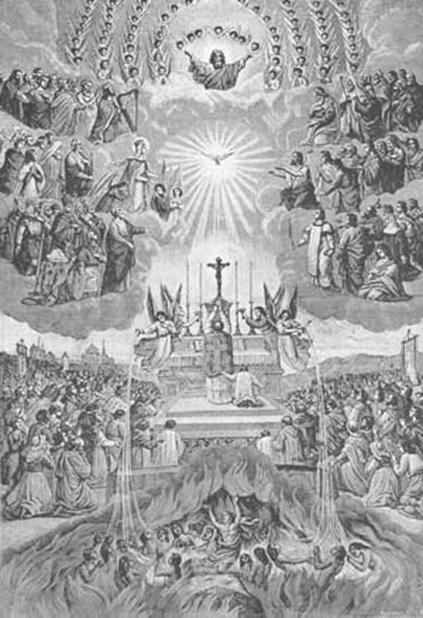
\includegraphics[scale=0.85]{gambar/purgatory2.jpg}
\end{center}

%\vspace{1cm}

\begin{center}
{\PTsmaller {Kasih, kerendahan hati, dan menurut pada kehendak Allah }}
\end{center}

\setlength{\parindent}{1cm}
\pagestyle{plain}
\begin{center}
%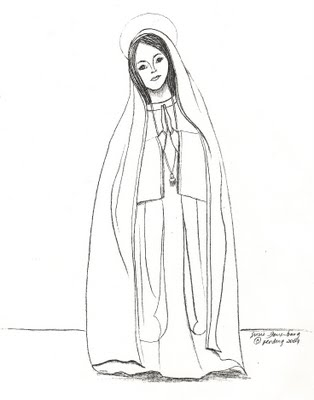
\includegraphics[scale=0.25]{gambar/Mary-Coloring-5.jpg}
\end{center}
\chap{Maria Sebagai Pola Hidup Orang Beriman\\
 \textit{P. Josep Susanto Pr}}

\section*{Inkarnasi}

\small
Misteri inkarnasi (natal) bukan cuma soal Sabda yang menjadi daging (manusia) atau  Allah yang mendatangi manusia untuk menebus umat manusia, melainkan misteri itu bisa kita lihat dan renungkan lebih dalam lagi yaitu Allah yang berinisiatif untuk bersatu dengan ciptaanNya secara definitif supaya ciptaanNya bersatu dengan Dia. Di sinilah terjadi peristiwa iman-wahyu : Proses Membuka diri (bdk. Yoh 1:1)
\begin{quote}
\textit{Pada mulanya adalah Firman; Firman itu bersama-sama dengan Allah dan Firman itu adalah Allah}
\end{quote}

Dalam peristiwa inkarnasi, Kristus, Sang Putra Allah, menjadi senasib dengan manusia, membuat ke-AllahanNya yang tidak terbatas menjadi seolah-olah terbelanggu dan berdiam dalam kemanusiaanNya, dengan segala kelemahan dan ketebatasanNya. Dalam hal ini Santo Agustinus mengatakan : Dia yang adalah Allah Putra, mengosongkan diriNya, dan mengambil rupa seorang hamba, namun Ia tidak kehilangan ke-AllahanNya.
	
Inkarnasi, Allah yang menjadi manusia, adalah suatu rencara besar Allah bagi manusia (Luk 2:10-14). Rencana ini tidak pernah bisa dilepaskan dari sejarah keselamatan manusia sejak manusia pertama kali jatuh ke dalam dosa.
(bdk. Ibr 1:1-2).
\begin{quote}
\textit{Setelah pada jaman dahulu Allah berulang kali dan dalam pelbagai cara berbicara kepada nenek moyang kita dengan perantaraan nabi-nabi, maka pada zaman akhir ini Ia telah berbicara kepada kita dengan perantaraan AnakNya, yang telah Ia tetapkan sebagai yang berhak menerima segala yang ada.}
\end{quote}

\section*{Maria diikutsertakan dalam Rencana Allah}

Setiap manusia dilibatkan oleh Allah dalam rencana keselamatan. Seperti kita ketahui cerita dan riwayat para nabi (Yesaya, Yeremia, Samson, Daud, Ishkak, dll). Dalam hal ini Maria mendapatkan peran yang sangat penting demi terjadinya kehendak Allah tersebut. Maria dipilih oleh Allah menjadi ibu Mesias.

Selama ini yang sering kita dengar dan renungkan mungkin hanya Maria akan mengandung seorang bayi, dan bayi itu anak Allah. Tetapi kalau kita memahaminya dari sudut pandang orang Yahudi tentunya tugas ini menjadi dua kali lebih berat dari pada yang kita bayangkan. Orang Yahudi sangat kental tradisi keagamaanNya. Orang Yahudi pada jaman Yesus bahkan sampai sekarang, menanti-nantikan hadirnya seorang Mesias, Juru Selamat. Sebagaimana janji Allah kepada Daud, Raja Israel, Allah akan membangkitkan seseorang dari keturuan Daud (dibaca : akan lahir dari keturunan Daud), dan akan menjadi raja bagi bangsa Israel, dan kerajaanNya akan jaya selamanya dan tidak akan pernah berakhir.

Sebagai seorang Yahudi yang saleh, Maria tentunya juga hidup dalam pengharapan yang sama dengan harapan orang-orang sebangsanya. Dalam peristiwa Maria menerima kabar Gembira dari Malaikat sebenarnya Maria mengalami dua keterkejutan sekaligus kebahagian.
\normalsize

Keterkejutan yang pertama adalah ternyata Mesias seorang tokoh yang sudah ditunggu-tunggu oleh seluruh bangsanya akan muncul. Harapan besar itu segera terwujud. Segala penderitaan Israel karena penjajahan dan morat marit pemerintahan pada waktu itu akan segera berakhir dengan hadirnya seorang mesias.

Keterkejutan yang kedua adalah ternyata mesias ini akan hadir ke dunia melalui rahimnya sendiri. Seperti yang sudah sering kita dengar, hal ini tentu tidak mudah bagi Maria yang nota bene masih sangat muda waktu itu.

Sisi yang kita mau kupas dalam kesempatan ini adalah pergulatan Maria ketika ia tahu bahwa yang dikandungnya adalah seorang tokoh besar yang sudah dinanti-nantikan dan diharap-harap oleh banyak orang. Orang Israel mengira Mesias akan lahir dari rahim seorang perempuan dari kalangan kerajaan, yang jelas-jelas keturunan Raja Daud. Sementara Maria hanya perempuan biasa. Bisa kita bayangkan sejak semula Maria sudah sadar akan penolakan bangsaNya terhadap Putranya ini. Akan terjadi tegangan antara pengharapan orang-orang sebangsanya dengan kenyataan apa yang dikehendaki oleh Yesus. Dan sepertinya penolakan terhadap Yesus Sebagai Sang mesias sungguh-sungguh terjadi.

Seperti kita tahu mendidik anak bukanlah pekerjaan yang mudah. Anak adalah titipan Tuhan di mana seorang ibu mempunyai tugas untuk mendidik dan membesarkannya dengan penuh kasih sayang dan pengorbanan yang tidak sedikit.

Dalam kasus Maria, hal ini menjadi sangat tidak mudah. Bisa dibayangkan bagimana sikap dan kelakuan Yesus setelah besar kalau Maria salah mendidiknya. Tugas Maria tidak berhenti ketika ia mengandung dan melahirkan Yesus. Tugas Maria seperti dikatakan dalam Injil adalah mendidik Yesus, memperkenalkan Yesus pada bait Allah, memperkenalkan Yesus pada tradisi bangsanya, mendampingi Yesus, bahkan sampai menemani di kaki Salib.

Senjata Maria adalah Doa. Menghadapi tugas yang tidak mudah itu Maria mempunyai kekuatan yaitu kesadaran bahwa Allah pasti akan mendampingi dia dalam segala hal. Doa Maria sudah sering kita doakan seperti Ibadat Sore yaitu dalam Kidung Maria.
(Luk 1:46-55) Dalam Kidung Maria sebetulnya terkandung iman Maria yang sangat dalam, yaitu Allah yang selalu setia pada perjanjianNya. Hidup kita ini didasari oleh perjanjian antara Allah dan manusia, di mana Allah akan memberikan berkat melimpah kepada manusia yang senantiasa percaya dan berpegang teguh padaNya. Dan dalam perjanjian itu Allah selalu setia sedangkan manusia seringkali lupa dan tidak setia dengan perjanjian tersebut. Namun Allah sebagai pihak yang dirugikan berkali-kali memperbaharui perjanjianNya dengan manusia dengan harapan manusia akan berubah. Di atas ketidaksetiaan manusia, Allah tetap setia.

\section*{Relevansi kita sekarang:}

Sebagai biarawati ataupun imam, kita sering mendapat penugasan-penugasan dari para pemimpin kita. Mungkin beberapa penugasan adalah hal yang tidak mudah ataupun yang tidak pernah kita bayangkan sebelumnya. Bahkan dalam pengalaman ada penugasan-penugasan yang sepertinya dalam hati kita mau nya kita tolak entah karena kita tidak suka, tugas itu terlalu berat, atau pun alasan lainnya.

Dalam situasi ini kita mungkin bisa mencontoh pengalaman Maria, yaitu melihat tugas itu dalam kacamata seluruh sejarah keselamatan Allah bagi manusia. Artinya setiap manusia menjadi rekan kerja Allah dalam mewujudkan keselamatan bagi dirinya dan sesamanya. Mungkin mendengar hal itu kita menjadi minder dan kecil hati dengan bertanya : Siapakah diri kita, kok bisa menyelamatkan seluruh dunia?

Dalam hal ini kita perlu ingat, Kerajaan Allah justru bermula dari hal-hal kecil dan sederhana yang hampir tidak diperhatikan dan diperhitungkan orang lain. Lagi-lagi Maria bisa menjadi contoh bagi diri kita untuk berani mengatakan :  \textbf{“Terjadilah padaku menurut kehendakMu.”}

\sumber{http://www.imankatolik.or.id}
\chap{Kuasa Doa Satu Salam Maria}

\begin{quote}
\textit{Salam Maria, penuh rahmat, Tuhan sertamu,
terpujilah engkau di antara wanita, dan terpujilah buah tubuhmu, Yesus.
\\{~}\\
Santa Maria, Bunda Allah, doakanlah kami yang berdosa ini,
sekarang dan waktu kami mati. Amin.}
\end{quote}

Jutaan umat Katolik biasa mendaraskan Salam Maria. Sebagian mendaraskannya dengan begitu cepat, bahkan tanpa memikirkan kata-kata yang mereka ucapkan. Pernyataan-pernyataan berikut ini semoga dapat membantu kita mendaraskannya dengan lebih khusuk.
 
Satu Salam Maria yang didaraskan dengan baik memenuhi hati Bunda Maria dengan sukacita dan memperolehkan bagi diri kita sendiri rahmat-rahmat luar biasa yang tak terkatakan, yang ingin dilimpahkan Bunda Maria kepada kita. Satu Salam Maria yang didaraskan dengan baik memperolehkan bagi kita jauh lebih banyak rahmat daripada seribu Salam Maria yang didaraskan secara asal.
 
Doa Salam Maria bagaikan suatu tambang emas di mana kita senantiasa dapat menggali darinya tanpa ia pernah menjadi habis. Sulitkah mendaraskan Salam Maria dengan baik? Yang kita perlukan hanyalah belajar memahami nilai dan artinya.
 
St. Hieronimus mengatakan bahwa “kebenaran yang terkandung dalam Salam Maria begitu agung dan luhur, begitu mengagumkan, hingga tak ada manusia atau pun malaikat yang dapat memahami sepenuhnya.”
 
St. Thomas Aquinas, Pujangga Gereja yang terkemuka, 'yang paling bijaksana di antara para kudus dan yang paling kudus di antara para bijaksana', seperti dinyatakan oleh Paus Leo XIII, berkhotbah selama 40 hari lamanya di Roma hanya tentang Salam Maria, membuat para pendengarnya terpesona serta penuh sukacita.
 
Pastor F. Suarez, seorang imam Yesuit yang terpelajar dan kudus, ketika sedang menghadapi ajal menyatakan bahwa dengan senang hati ia akan menyerahkan seluruh dari banyak buku berbobot yang ia tulis, juga seluruh karya sepanjang hidupnya, demi mendapatkan ganjaran dan jasa dari satu doa Salam Maria yang didaraskan dengan khusuk dan tulus.


St. Mechtilda, yang sangat mengasihi Bunda Maria, suatu hari sedang berusaha keras untuk menggubah sebuah doa yang indah untuk menghormati Bunda Maria. Bunda Maria menampakkan diri kepadanya, dengan tulisan emas di dadanya: “Salam Maria penuh rahmat.” Santa Perawan berkata kepadanya, “Berhentilah, anakku terkasih, dari usahamu itu, oleh sebab tidaklah mungkin engkau dapat menggubah suatu doa yang dapat memberiku sukacita dan kebahagiaan seperti Salam Maria.”


Seorang pria memperoleh sukacita luar biasa dengan mendaraskan Salam Maria secara perlahan-lahan. Santa Perawan menampakkan diri kepadanya dengan tersenyum dan mengatakan kepadanya hari serta jam bilamana ia akan meninggal, serta memperolehkan baginya kematian yang paling kudus dan bahagia. Setelah kematiannya, sekuntum bunga bakung putih yang indah tumbuh dari mulutnya. Pada daun-daun bunganya tertulis “Salam Maria”.
 
Cesarius menceritakan kisah serupa. Seorang biarawan yang rendah hati dan kudus tinggal di sebuah biara. Daya tangkap dan daya ingatnya begitu lemah hingga ia hanya dapat menghafalkan satu doa saja, yaitu “Salam Maria”. Setelah kematiannya, sebatang pohon tumbuh di atas kuburnya dan pada semua daun-daunnya tertulis: “Salam Maria”.
 
Kisah-kisah indah berikut ini menunjukkan kepada kita betapa tinggi nilai devosi kepada Bunda Maria dan betapa besar kuasa doa Salam Maria yang didaraskan dengan khusuk.
 
Setiap kali kita mengucapkan Salam Maria, kita mengulangi kata-kata yang sama yang diucapkan Malaikat Agung St. Gabriel pada waktu menyampaikan salam kepada Maria pada Hari Kabar Sukacita, yaitu ketika ia menjadi Bunda Putra Allah.
 
Begitu banyak rahmat dan sukacita yang memenuhi jiwa Maria saat itu.
 
Sekarang, pada saat kita mendaraskan Salam Maria, kita mempersembahkan sekali lagi segala rahmat dan sukacita tersebut kepada Bunda Maria dan ia menerimanya dengan bahagia yang mendalam.
 
Sebagai balasnya, ia membagikan sukacitanya itu kepada kita.
 
Suatu ketika, Yesus meminta St. Fransiskus Asisi untuk memberi-Nya sesuatu. Orang kudus itu menjawab, “Tuhan terkasih, aku tak dapat memberi-Mu apa-apa lagi, sebab aku telah memberikan segalanya untuk-Mu, yaitu segenap cintaku.”
 
Yesus tersenyum dan berkata, “Fransiskus, berikan pada-Ku segenap cintamu itu lagi dan lagi, setiap kali, cintamu itu mendatangkan kesukaan yang sama bagi-Ku.”
 
Demikian juga dengan Bunda kita terkasih. Setiap kali kita mendaraskan Salam Maria, Bunda Maria menerima dari kita segala sukacita dan kebahagiaan yang sama seperti yang ia terima dari perkataan St. Gabriel.
 
Allah yang Mahakuasa telah menganugerahkan kepada Bunda-Nya yang Terberkati segala kemuliaan, keagungan, dan kekudusan yang diperlukan untuk menjadikannya Bunda-Nya Sendiri yang paling sempurna.
 
Namun demikian, Ia juga menganugerahkan kepada Bunda-Nya segala pesona, cinta, kelemah-lembutan serta kasih sayang yang diperlukan untuk menjadikannya Bunda kita yang paling terkasih. Bunda Maria adalah sungguh-sungguh dan benar-benar Bunda kita.
 
Seperti anak-anak lari kepada ibunya ketika menghadapi bahaya untuk minta perlindungan, demikian juga patutlah kita lari segera dengan keyakinan tak terbatas kepada Maria.
 
St. Bernardus dan banyak para kudus lainnya mengatakan bahwa tak pernah sekali pun terdengar pernah terjadi di suatu waktu atau pun tempat bahwa Bunda Maria menolak mendengarkan doa anak-anaknya yang di bumi.
 
Mengapakah kita tidak menyadari kebenaran yang sangat menghibur hati kita ini? Mengapakah kita menolak cinta dan penghiburan yang ditawarkan oleh Bunda Allah yang Manis kepada kita?
 
Adakah sikap acuh kita yang mengerikan, yang menjauhkan kita dari pertolongan dan penghiburan yang sedemikian itu?
 
Mengasihi dan mengandalkan Maria berarti berbahagia di dunia sekarang ini dan berbahagia kelak di Surga.


Dr. Hugh Lammer adalah seorang Protestan fanatik, dengan prasangka-prasangka kuat menentang Gereja Katolik. Suatu hari ia menemukan suatu penjelasan tentang Salam Maria dan membacanya. Ia begitu terpesona olehnya hingga mulai mendaraskannya setiap hari. Tanpa disadarinya, segala antipati dan kebenciannya terhadap Gereja Katolik mulai lenyap. Ia menjadi seorang Katolik, seorang imam yang kudus dan profesor Teologi Katolik di Breslau.


Seorang imam diminta datang ke sisi pembaringan seorang yang sedang menghadapi ajal dalam keputusasaan oleh karena dosa-dosanya. Namun demikian, orang itu bersikukuh menolak mengakukan dosa-dosanya. Sebagai usahanya yang terakhir, imam meminta si sakit agar setidak-tidaknya ia mendaraskan Salam Maria. Sesudah mendoakan Salam Maria, pria malang itu mengakukan dosanya dengan tulus dan meninggal dengan kudus.
 
Di Inggris, seorang imam paroki diminta untuk pergi menemui seorang wanita Protestan yang sedang sakit parah dan rindu menjadi seorang Katolik. Ketika ditanya apakah ia pernah pergi ke Gereja Katolik, atau apakah ia pernah belajar dari umat Katolik, atau apakah ia membaca buku-buku Katolik, ia menjawab, “Tidak, tidak pernah.” Sejauh yang dapat diingatnya ialah - ketika masih kanak-kanak - ia belajar dari seorang gadis kecil tetangga yang Katolik doa Salam Maria, yang kemudian dilakukannya setiap malam. Wanita itu kemudian dibaptis dan sebelum meninggal boleh menikmati kebahagian menyaksikan suami dan anak-anaknya dibaptis juga.


St. Gertrude mengatakan dalam bukunya, “Wahyu” bahwa ketika kita mengucap syukur kepada Tuhan atas rahmat-rahmat yang Ia berikan kepada seorang kudus tertentu, kita juga memperoleh bagian besar atas rahmat-rahmat tersebut.


\small
Jika demikian, rahmat-rahmat apakah yang tidak akan kita peroleh jika kita mendaraskan Salam Maria sementara kita mengucap syukur kepada-Nya atas segala rahmat tak terkatakan yang telah Ia anugerahkan kepada Bunda-Nya Maria?


\sumber{With Ecclesiastical Approval}
 
“. . . Satu Ave Maria (Salam Maria) yang didaraskan tanpa perasaan mendalam, tetapi dengan kehendak yang tulus dalam masa kekeringan, jauh lebih bernilai di hadapanku daripada satu Rosario penuh yang didaraskan di tengah penghiburan.”
 
\sumber{Bunda Maria kepada Sr. Benigna Consolata Ferrero}

 
“Seorang imam Yesuit yang kudus dan terpelajar, Pastor Suarez, memahami dengan begitu mendalam nilai Salam Malaikat (Salam Maria) hingga ia mengatakan bahwa ia akan dengan senang hati menyerahkan segala ilmu yang diperolehnya demi memperoleh ganjaran dan jasa satu Salam Maria yang didaraskan dengan pantas.”
 
\sumber{St. Louis De Montfort, Rahasia Rosario, hal. 48}
\normalsize
\chap{Meneladani Maria}

“Salam, hai engkau yang dikaruniai, Tuhan menyertai engkau”  Maria adalah seorang gadis desa, yang sederhana dan dipilih Allah untuk menunjukan karya kemuliaan dan kerahiman Allah kepada manusia. Mengapa Allah memilih Maria? Hanya Allah yang tahu. Tetapi dari telaah Kitab Suci: Allah selalu memilih/memakai yang lemah/sederhana/tersisih untuk melakukan karya-karya besar supaya hanya kemuliaan Tuhan yang nampak. Tuhan juga memilih kita orang berdosa untuk diselamatkanNya.


Maria sebagai manusia biasa juga ber-reaksi kaget/ terkejut/ ragu-ragu/ takut, pada mulanya tidak percaya ketika mendapat kinjungan dari Malaikat / utusan Tuhan sendiri, tetapi maria tidak berhenti dengan ketakutan dan kerahu-raguannya. Maria berusaha mencari jawaban dari si pembawa berita yaitu Malaikat Tuhan yang bernama Malaikat Agung Gabriel. Apakah kita pun mencari jawaban dari Tuhan ketika mengalami keraguan/bimbang dalam memutuskan sesuatu ?

“Tidak ada yang mustahil bagi Allah”  Secara manusia hamil tanpa berhubungan sex adalah tidak mungkin. Ini adalah karya Roh Kudus yang ingin menunjukan bahwa Allah sanggup melakukan segala sesuatu. Kita harus melihat ini dengan iman. Iman berarti kepercayaan dan penyerahan diri secara total kepada kehendak Allah. Maria adalah Musa baru dalam teladan iman dan penyerahan diri kepada Allah (Bdk. Abraham siap mengorbankan anak tunggalnya karena perintah Allah - Kej 22:1-11)

Maria menjadi teladan setiap orang beriman, terutama orang katolik, dalam iman dan kepercayaannya kepada Allah. Pengabdiaan Maria kepada Allah terungkap lewat sikap yang siap menerima tugas dan perintah Allah sekalipun akan berakibat penghinaan, penolakan dan bahaya kematian dari masyarakat sekitarnya pada waktu itu. “Sesungguhnya aku ini adalah hamba Tuhan; jadilah padaku menurut perkataanmu itu” (Lukas 1:38). Rencana penyelamatan Allah tidak akan terlaksana jika Maria tidak mengatakan “YA” kepada kehendak Allah. Kita diselamatkan oleh Yesus yang ada di dunia ini karena jawaban “YA” (FIAT) Maria itu.

“Malaikat itu meninggalkan Maria”  Allah membiarkan dan membebaskan Maria untuk melaksanakan tugas yang telah diutuskan kepadanya. Maria di hadapkan pada ketidakpastian dan ketidakjelasan panggilan Allah yang penuh dengan resiko. Kita pun diberi kebebasan oleh Allah untuk melakukan segala sesuatu sesuai dengan kehendakNYA atau kehendakku dengan segala resiko masing-masing. Apakah kita selalu memilih yang baik dan benar apapun resikonya?

Sama seperti Maria, Allah pun memilih kita bukan karena kita pandai/ kaya/ hebat/ cantik, tapi Allah selalu melihat hati; ketulusan/ ketaatan/ kerendahan hati/ kepasrahan kepada Allah yang ditunjukan Maria itulah yang selalu menjadi teladan bagi orang katolik. Mengapa kita yang dipilih? Hanya Tuhan yang tahu. Itulah tanda cinta dan kasih setia Tuhan pada kita manusia berdosa. Sudahkah kita bersyukur untuk itu?

Dengan iman dan penyerahan diri Maria kepada Allah, selain menjadi teladan kita, Maria, karena kedekatannya dengan Allah juga menjadi perantara orang katolik untuk menyampaikan segala permohanan kita kepada Yesus. Yesus dan Maria menjadi Adam dan Hawa baru untuk menebus dosa para leluhur kita di taman Firdaus. Yesus adalah sumber Rahmat dan Maria adalah perantara rahmat yang membuat kita lahir kembali dan mendapat tempat di surga.

Pribadi Maria dalam kehidupan orang katolik mendapat tempat yang istimewa. Penghormatan (devosi) Gereja Katolik kepada Maria dilakukan dengan beberapa hal, misalnya memperingati hari-hari penting Bunda Maria, berdoa Salam Maria dan Rosario, Novena Tiga Salam Maria, puji-pujian kepada Maria dan berziarah ke Gua Maria. Gereja menetapkan bulan Mei dan Oktober sebagai bulan penghormatan (devosi) kepada Bunda Maria. Dalam bulan-bulan ini akan banyak kegiatan di Gereja dan lingkungan/wilayah untuk menghormati Bunda Maria.

Doa Salam Maria bersumber dari ucapan salam dari Malaikat Utusan Allah kepada Maria (Salam Maria, penuh Rahmat, Tuhan besertamu) dan ungkapan Elisabeth ketika bertemu Maria (Terpujilah Engkau antara wanita dan terpujilah buah Tubuhmu: Yesus).

Keberadaan gua maria, patung maria bukan untuk menggeser atau menyamakan posisi Yesus. Patung atau gambar bukan dewa yang disembah. Orang katolik tidak menyembah berhala, patung dll. Itu hanyalah sarana untuk lebih mudah berkonsentrasi dalam berdoa, seperti halnya kita melihat foto. Tujuan utama adalah satu yaitu Tuhan Yesus sendiri. Maria adalah pengantara untuk menyampaikan segala permohonan, keinginan, menyatukan, mendekatkan kita kepada Putranya Yesus.
\chap{Perjalanan Menuju Iman Katolik}
\begin{quote}
“Ia membuat segala sesuatu indah pada waktunya, bahkan Ia memberikan kekekalan dalam hati mereka. Tetapi manusia tidak dapat menyelami pekerjaan yang dilakukan Allah dari awal sampai akhir.” (Pengkhotbah 3 : 11)
\end{quote}

Tak pernah terbayang sebelumnya, kalau pada akhirnya aku akan memilih untuk menjadi seorang Katolik. Ini merupakan keputusan terbesar dalam hidupku setelah pernikahan. Sekali mengatakan “Ya”, berarti untuk selamanya!!

Setelah melalui perjalanan yang panjang dengan liku-likunya, yang terkadang penuh duri dan terasa amat menyakitkan, serta acap kali menemui persimpangan jalan hingga membuatku cukup mengalami depresi, kini aku, dengan langkah pasti dan kepala tegap terangkat, dapat mengarahkan hatiku untuk melangkah memasuki Gereja Katolik. Ya, Gereja Katolik!

Gereja Katolik yang dahulunya sangat bertentangan dengan hatiku, dengan pikiranku, dengan seluruh keberadaanku sebagai seorang Protestan.
Dulu, aku sangat membenci doktrin-doktrin Katolik, khususnya ajaran mengenai ‘Maria’.

Bagiku, Maria adalah penghalang utama orang Katolik untuk mendekat lebih lagi kepada Yesus. Apapun yang orang Katolik jelaskan, termasuk pacarku sendiri, tentang doktrin Maria, otakku tidak bisa menerimanya, hatiku selalu memberontak dengan keras. Bagiku doktrin Maria hanyalah buatan manusia, karangan Paus semata!
Salah satu penyebab kebencianku terhadap Maria adalah juga karena kegemaranku membaca buku-buku rohani yang berhubungan dengan alam roh. Aku pernah membaca sebuah buku yang ditulis oleh seorang mantan penyihir dari Afrika, bernama “Mukendi”. Di situ dikatakan bahwa ketika Allah mengusir Lucifer dari Firdaus, ia tidak hanya terlempar seorang diri saja, tetapi bersama pengikut-pengikutnya, dan para pengikutnya itu tersebar ke berbagai tempat. 

Ada yang terjatuh ke dalam laut, dan menjadi penguasa lautan. Kebetulan malaikat penguasa laut ini bernama “Maria Marguella”, ia sering mengaku sebagai Maria ibu Yesus. Dan menurut Mukendi, orang yang berdoa kepada Maria, secara tidak langsung mereka sedang berdoa kepada malaikat penguasa lautan ini.

Ada juga malaikat yang jatuh ke langit, dan menjadi penguasa langit, dibawah kakinya terdapat tulisan: Rosa, yang berarti “naga”. Dan orang yang berdoa Rosario secara tidak langsung juga mereka sesungguhnya sedang berdoa kepada malaikat penguasa langit tersebut.
Masih banyak hal lainnya yang membuatku semakin membenci Maria, dan mengasihani orang-orang Katolik.

Aku menelan seluruh isi buku itu bulat-bulat, tanpa ada sedikit pun perlawanan dari dalam diriku. Sekarang buku itu sudah tidak ada lagi, bukan karena hilang, atau kubuang, tetapi, (sekarang aku baru menyesal), karena buku tersebut sudah kuberikan kepada seseorang yang tidak kukenal, yang sudah hampir menemui ajalnya karena sakit berat.

Aku pernah bertanya kepada pacarku yang seorang Katolik:
“Kalau memang tujuan dari setiap penampakan Maria itu adalah membawa orang untuk lebih dekat lagi kepada Yesus, kenapa tidak Yesus sendiri saja yang langsung menampakan diriNya kepada orang-orang, kenapa harus Maria? Apa mungkin Maria yang adalah manusia biasa, sama seperti kita, bisa dengan mudahnya naik turun Surga hanya untuk menampakkan dirinya?”

Sementara aku sedang mengajukan pertanyaan itu, di dalam pikiranku sendiri tiba-tiba muncul gambaran tentang penampakan Musa dan Elia, ketika Yesus dan ketiga muridNya naik ke gunung yang tinggi.
Matius 17:3 Maka nampak kepada mereka Musa dan Elia sedang berbicara dengan Dia.

Kemudian aku mendengar pacarku itu menjawab:
“Mungkin saja, kalau itu memang sesuai dengan kehendak Tuhan. Contohnya Musa dan Elia yang menampakan diri kepada Yesus!”
Aku terdiam dan jadi heran sendiri. Bukan hanya karena jawaban dari pacarku itu, tapi terutama tentang gambaran yang tadi tiba-tiba saja muncul di dalam pikiranku, seolah-olah aku sudah diberitahu jawabannya terlebih dahulu sebelum pacarku menjawab.

Kisah cintaku semasa pacaran banyak dihiasi dengan pertengkaran seputar doktrin Katolik, terutama doktrin Maria ini.
Aku juga pernah berkata kepada pacarku kemudian, yang sekarang sudah menjadi suami tercintaku:
“Kenapa sih dalam doa Rosario, Salam Maria didoakan sampai 10 kali, sementara doa Bapa kami cuma satu kali saja?”

Tanpa menunggu jawaban dari pacarku itu, aku kembali berkata dengan ketus:
“Dasar Maria egois! serakah! Maunya dia yang paling banyak didoakan!”
Saat itu pacarku masih sabar dalam menghadapi perlawananku, yang kalau kupikir sekarang, sudah amat keterlaluan.

Tapi, ada suatu waktu dia sudah tidak dapat lagi menahan kemarahannya, karena mendengar penghinaanku terhadap Bunda Maria. Aku sudah lupa bagaimana kejadiannya saat itu, tapi yang aku tidak dapat lupakan adalah tanggapannya yang sangat keras:
“Yayang boleh sepuasnya menghina Koko, tapi jangan sekali-kali Yayang menghina Mama Koko, apalagi Mama yang sangat Koko hormati!”

Setelah berkata seperti itu, dia pun pergi dengan penuh kemarahan, meninggalkan aku sendiri yang pada saat itu masih juga dapat tersenyum, karena pikirku:
“Siapa juga yang menghina mamanya, orang yang aku hina Maria, bukan mamanya!”
Tapi sekarang aku sudah mengerti bahwa yang dimaksud pacarku waktu itu adalah Maria sebagai mamanya, sebagai ibu rohaninya.

Saat tergantung di kayu salib, Yesus menyerahkan ibuNya kepada murid terkasihNya, Yohanes, dengan berkata kepada ibuNya: “Ibu, inilah anakmu!”, dan kepada murid terkasihNya: ” Inilah ibumu!”, dan mulai saat itu Yohanes menerima Maria di dalam rumahnya. (Yoh 19 : 26-27)
Karena kita juga adalah murid terkasih Yesus, maka ibuNya pun menjadi ibu kita. Bahkan dalam Ibrani 2 : 11-12, Yesus menyebut kita adalah saudara-saudaraNya.
\begin{quote}
Ibrani 2 : 11 Sebab Ia yang menguduskan dan mereka yang dikuduskan, mereka semua berasal dari Satu; itulah sebabnya Ia tidak malu menyebut mereka saudara,
Ibrani 2 : 12 Kata-Nya: “Aku akan memberitakan nama-Mu kepada saudara-saudara-Ku, dan memuji-muji Engkau di tengah-tengah jemaat,”
\end{quote}

Meski bibirku tersenyum mendengar kata-kata pacarku yang menyebut Maria sebagai mamanya, tapi sesungguhnya hatiku porak poranda. Aku langsung berlari masuk ke dalam kamar dan menangis sejadi-jadinya.
Aku bertanya kepada Tuhan:
“Mengapa Tuhan \ldots , mengapa harus aku yang mengalami hal seperti ini? Engkau tahu kalau aku ini paling anti Katolik… Tak pernah sekalipun dalam doaku, aku memohon kepadaMu untuk mengirimkan padaku seorang pacar Katolik…! Lalu mengapa Kau malah mengirimkan padaku seseorang yang bahkan sangat kuat dalam iman Katoliknya? Siapakah itu Maria? Tolong Tuhan, tunjukkan padaku siapakah itu Maria?”

Pada suatu hari, aku melihat sebuah buku dari daftar buku di perpustakaan kantorku. Buku itu sangat menarik minatku. Aku sudah sangat sering mendengar nama dan karya sungguh luar biasa yang dikerjakan tokoh utama dalam buku itu, yaitu : Bunda Theresa, tapi baru kali ini aku berminat untuk membaca seluruh kisah kehidupannya.

Aku sungguh terharu dan kagum menyaksikan kasih yang dinyatakan oleh Bunda Theresa kepada orang-orang kusta di Kalkuta, India. Sekalipun dia tidak pernah mengatakan tentang Yesus kepada orang-orang malang yang dilayaninya, tetapi pada akhirnya banyak dari mereka yang percaya kepada Yesus, karena melihat perbuatan nyata penuh kasih yang dilakukan Bunda Theresa.

Ini barulah kesaksian yang hidup. Kesaksian yang sesungguhnya!
Aku merasa heran, mengapa orang Katolik bisa melakukan hal luar biasa seperti ini? Mengapa mereka memiliki kasih yang sedemikian nyatanya, hingga seolah-olah Yesus sendiri yang berkerja dalam mereka, dan nampak dalam setiap laku mereka?

Aku juga melihat bahwa Bunda Theresa memiliki hubungan yang akrab dengan Yesus. Bagaimana ini bisa terjadi…? Bukankah seharusnya Maria menjadi penghalang hubungan mereka dengan Yesus? Padahal Bunda Theresa juga sering berdoa Rosario, berarti dia juga memiliki hubungan yang dekat dengan Maria? Lalu, apa sebenarnya yang salah dalam buku ini?

Setelah membaca habis buku itu, aku duduk termenung. Aku mulai membayangkan perjalanan Bunda Theresa yang pastinya penuh perjuangan, melayani orang-orang berpenyakitan dan menjadi sampah masyarakat. Bukan hanya itu saja, perjuangannya lebih terasa berat lagi, karena dia melayani bukan di negaranya sendiri, tetapi di negara orang.

Oleh karena kasihnya kepada Yesus, yang dinyatakan kepada mereka yang malang, Bunda Theresa mampu melewati semuanya itu dengan penuh kesabaran dan ketekunan.
Aku jadi teringat dengan perkataan Yakobus dalam suratnya:Yakobus 2, 
\begin{quote}
2:14 Apakah gunanya, saudara-saudaraku, jika seorang mengatakan, bahwa ia mempunyai iman, padahal ia tidak mempunyai perbuatan? Dapatkah iman itu menyelamatkan dia?

2:15 Jika seorang saudara atau saudari tidak mempunyai pakaian dan kekurangan makanan sehari-hari,

2:16 dan seorang dari antara kamu berkata: “Selamat jalan, kenakanlah kain panas dan makanlah sampai kenyang!”, tetapi ia tidak memberikan kepadanya apa yang perlu bagi tubuhnya, apakah gunanya itu?

2:17 Demikian juga halnya dengan iman: Jika iman itu tidak disertai perbuatan, maka iman itu pada hakekatnya adalah mati.

2:18 Tetapi mungkin ada orang berkata: “Padamu ada iman dan padaku ada perbuatan”, aku akan menjawab dia: “Tunjukkanlah kepadaku imanmu itu tanpa perbuatan, dan aku akan menunjukkan kepadamu imanku dari perbuatan-perbuatanku.”

2:19 Engkau percaya, bahwa hanya ada satu Allah saja? Itu baik! Tetapi setan-setan pun juga percaya akan hal itu dan mereka gemetar.

2:20 Hai manusia yang bebal, maukah engkau mengakui sekarang, bahwa iman tanpa perbuatan adalah iman yang kosong?

2:21 Bukankah Abraham, bapa kita, dibenarkan karena perbuatan-perbuatannya, ketika ia mempersembahkan Ishak, anaknya, di atas mezbah?

2:22 Kamu lihat, bahwa iman bekerjasama dengan perbuatan-perbuatan dan oleh perbuatan-perbuatan itu iman menjadi sempurna.

2:23 Dengan jalan demikian genaplah nas yang mengatakan: “Lalu percayalah Abraham kepada Allah, maka Allah memperhitungkan hal itu kepadanya sebagai kebenaran.” Karena itu Abraham disebut: “Sahabat Allah.”

2:24 Jadi kamu lihat, bahwa manusia dibenarkan karena perbuatan-perbuatannya dan bukan hanya karena iman.
Jadi, apalah gunanya kotbah yang berkobar-kobar, jika tidak disertai dengan perbuatan nyata penuh kasih?
\end{quote}

Setelah hari itu, aku makin penasaran dengan kisah hidup orang-orang Katolik. Aku mulai melirik website yang berbau Katolik di internet, dan aku menemukan kisah para Santa/Santo, orang-orang yang dianggap kudus oleh Gereja Katolik, karena teladan hidupnya yang luar biasa, atau karyanya yang telah membawa suatu kesaksian dalam pertumbuhan iman Katolik.

Banyak daftar nama-nama Santa/Santo di sana. Tetapi aku menemukan seorang Santa yang membuat mataku semakin terbuka lebar dan membuat keherananku semakin menjadi-jadi. Tak pernah sekalipun kusangka sebelumnya akan menemukan yang seperti ini di dalam sejarah Gereja Katolik. Bagiku orang-orang Katolik hanyalah boneka-boneka hidup yang datang dan pulang Gereja bukan karena kerinduan untuk mencari Tuhan, tapi hanya sebatas kewajiban. Mereka pulang tak ada bedanya dengan ketika mereka datang. Aku berpikir mereka hanya patuh pada peraturan yang dibuat Paus saja. Jarang sekali aku menemukan teman-temanku Katolik yang mengerti Alkitab. Bahkan, yang lebih parahnya lagi, ada juga yang bingung ketika mencari letak dari kitab tertentu dalam Alkitab!

Tapi di sini, dalam buku harian Santa ini, aku menemukan sesuatu yang sangat berbeda. Sungguh kebalikan 180 derajat dari apa yang kupikirkan mengenai orang Katolik. Seseorang yang begitu akrab dengan Yesus, sampai seolah-olah Yesus benar-benar nampak di dalam kehidupan sehari-hari Santa ini. Ia melihat dan berbicara kepada Yesus seperti ia sedang melihat dan berbicara dengan sahabatnya sendiri. Begitu nyata dan alami.

Santa ini bernama St. Faustina Kowalska, dan dia mendapat gelar sebagai: RASUL KERAHIMAN ILAHI.
Sejak saat itu, aku sudah mengetahui nama apa yang kelak akan kupakai sebagai nama baptisku: “Faustina”.

Aku merasakan hatiku semakin terbuka terhadap Gereja Katolik, beserta berbagai rahasianya yang kian menguak di depan mataku. Sementara hatiku kian menggelegak dalam kerinduan pencarian akan kebenaran yang tersembunyi dalam Gereja Katolik, seperti sedang mencari sebuah harta karun yang terkubur dalam gua-gua mengerikan, demikian hatiku menjelajah kian jauh menelusup dalam gudang rahasia Gereja Katolik. Namun, di sisi yang lain dalam otakku masih juga tak dapat memahami tentang doktrin Maria, api penyucian, dan persekutuan dengan para kudus!

Mengapa orang Katolik harus berdoa kepada Maria, dan menjadikannya perantara kepada Yesus? Mengapa tidak langsung saja berbicara kepada Yesus, kenapa harus melalui jalan yang memutar? Apa fungsi doa Rosario yang diulang-ulang? Mengapa juga mereka sering berdoa pada Santa atau Santo, orang-orang yang sudah mati? Dan masih banyak lagi pertanyaan-pertanyaan yang membuat otakku menjadi linglung!

Aku terus mencari dan mencari, berusaha menemukan kebenaran yang telah, oh belum, hanya baru separuh terlihat. Keharuman yang baru sedikit, sangat sedikit tercium olehku. Keharuman serta keindahan yang secara perlahan-lahan mengerogoti kengerianku terhadap sosok Gereja Katolik.

Aku mulai membaca lebih dalam lagi, dari sejarah Gereja Katolik, sejarah pohon natal, lagu Malam Kudus, hingga sejarah Alkitab, semuanya itu dimulai oleh Katolik. Ya, orang-orang Katolik! Gereja Katolik yang berani dengan jelas menyatakan bahwa dirinya adalah Gereja yang didirikan oleh Tuhan Yesus sendiri melalui Rasul Petrus, Paus pertama dalam sejarah Gereja Katolik! Dan telah melewati berabad-abad, baik dalam masa tenang maupun melewati masa-masa gelap, tetap berdiri kokoh seperti batu karang di tengah terjangan badai dunia!
Matius 16:18 Dan Aku pun berkata kepadamu: Engkau adalah Petrus dan di atas batu karang ini Aku akan mendirikan jemaat-Ku dan alam maut tidak akan menguasainya.

Pacarku juga mulai mengirimiku banyak artikel tentang Bunda Maria. Tidak seperti dulu, kini hatiku makin melunak dalam memandang Maria sebagai seseorang yang sangat dihormati oleh orang Katolik.

Hingga suatu hari, pacarku memberikan kepadaku sebuah buku yang merupakan serentetan peluru senapan yang berhasil menjebol dinding pertahananku. Buku yang mengisahkan kepindahan seorang pendeta Presbytarian, seorang anti Katolik yang menganggap orang-orang Katolik adalah orang-orang malang yang perlu diselamatkan, dan menyebut Gereja Katolik sebagai pelacur dari Babilonia. Menjadi seorang Katolik, seorang pengikut Paus yang luar biasa dalam pengetahuannya tentang ajaran Katolik.

Dalam bukunya yang berjudul : “Rome Sweet Home (Roma Rumahku)”, Scott dan isterinya, Kimberly, menceritakan dengan detil, bagaimana mereka bisa sampai mengakui Gereja Katolik sebagai rumah sejatinya. Bagaimana, dengan rinci dan penuh ketelitian, serta mengacu pada ayat-ayat dalam Alkitab, Scott menjabarkan bahwa ajaran Katolik sangatlah Alkitabiah. Bagaimana Kimberly, baik dalam segi perasaan dan pandangannya terhadap ajaran Katolik, khususnya Maria, sama persis dengan apa yang telah dan sedang kurasakan serta pikirkan sekarang. Dan bagaimana cara dia mengatasinya, sungguh membuatku semakin mengerti dan menjadi semakin berkobar-kobar dalam kerinduanku meneguk habis setiap kebenaran yang disodorkan Alkitab mengenai ajaran Gereja Katolik!

Setiap Minggu, aku dan pacarku pergi ke Gereja Katolik. Dulu aku sangat menganggap remeh setiap tata cara liturginya. Bagiku dulu, nyanyian dan segala hal yang mencakup tata cara ibadah, termasuk kotbah Romo, sangat membosankan!

Aku pernah mengejek pacarku yang setiap masuk dan keluar pintu Gereja selalu membungkukan badan, menghadap Altar Tuhan, kebetulan beberapa kali aku tepat berada di depannya, jadi aku secara spontan berkata: “Duh \ldots , nggak usah repot-repot nyembah aku!”

Dan dalam beberapa kesempatan, aku sengaja melakukan apa yang dilarang pacarku untuk dilakukan di dalam Gereja, terutama saat Misa berlangsung. Seperti misalnya, aku sengaja minum dari botol minum yang kubawa ketika Romo sedang berkhotbah! Aku melakukan itu, semata-mata hanya ingin menunjukan kepada pacarku kalau aku tidak terikat pada peraturan, yang kupikir, hanya merupakan peraturan-peraturan yang dibuat oleh manusia.

Tapi sekarang, aku sudah mengerti, kalau sesungguhnya ketaatan itu sangat penting. Satu hal yang tidak dapat iblis lakukan adalah ‘taat’!
Dan aku tidak mau disamakan dengan iblis! Yesus saja taat kepada BapaNya sampai mati…, sampai mati di kayu salib!

I Petrus 1:22 Karena kamu telah menyucikan dirimu oleh ketaatan kepada kebenaran, sehingga kamu dapat mengamalkan kasih persaudaraan yang tulus ikhlas, hendaklah kamu bersungguh-sungguh saling mengasihi dengan segenap hatimu.

Ketika hatiku mulai mengerti, aku dapat melihat setiap detil dalam tata cara liturgi sangatlah bermakna. Seperti membungkuk, bersujud, dan melagukan kata-kata, semuanya itu sungguh-sungguh memiliki arti yang mendalam. Mereka percaya bahwa Yesus sungguh hadir dalam setiap perayaan Ekaristi kudus. Bahwa Hosti yang berada di Altar adalah Yesus sendiri, bukan sekedar simbol dari tubuh dan darah Kristus, tapi sungguh-sungguh Yesus sendiri!

Oleh sebab itulah mengapa mereka sangat menghormati Altar kudus, karena di situlah Sang Raja kemuliaan bersemayam! Dan puncak dalam setiap perayaan Ekaristi adalah “Komuni”, di mana kita sungguh-sungguh dipersatukan kembali dengan Kristus. Sungguh misteri yang luar biasa, yang baru kutemukan dan baru kusadari keindahannya!

Demikianlah, sedikit demi sedikit, satu demi satu rahasia itu mulai tersingkap di hadapanku. Begitu manis dan menggairahkan, seolah menggugah kerinduanku untuk melahap lebih dan lebih lagi.

Aku terus melangkah dan melangkah, menapaki lembaran baru dalam perjalanan imanku, menyambut setiap kebenaran baru dengan penuh kekaguman. Namun, setiap kali berhadapan dengan doktrin Maria, aku kembali terbentur. Seakan-akan kakiku tertanam amat dalam, hingga sulit melangkah pada yang satu ini!

Tiap malam aku selalu bertanya kepada Tuhan:
“Siapakah itu Maria yang dihormati sedimikian rupa oleh orang Katolik?… Tolong Tuhan, tunjukanlah padaku, siapakah itu Maria, dan apa yang sepatutnya harus aku perbuat, agar aku tidak menyakiti hatiMu?”
Demikianlah aku terus bergumul dalam doaku untuk tahap pencarianku pada yang satu ini.

Suatu hari aku menemukan ayat dalam perjanjian lama yang menggambarkan tentang kebundaan Maria lewat Batsyeba, ibu dari raja Salomo. (1 Raja-raja) 

\begin{quote}
2:19 Batsyeba masuk menghadap raja Salomo untuk membicarakan hal itu untuk Adonia, lalu bangkitlah raja mendapatkannya serta tunduk menyembah kepadanya; kemudian duduklah ia di atas takhtanya dan ia menyuruh meletakkan kursi untuk bunda raja, lalu perempuan itu duduk di sebelah kanannya.

2:20 Berkatalah perempuan itu: “Suatu permintaan kecil saja yang kusampaikan kepadamu, janganlah tolak permintaanku.” Jawab raja kepadanya: “Mintalah, ya Ibu, sebab aku tidak akan menolak permintaanmu.”
\end{quote}

Di sini bunda ratu bertindak sebagai perantara permohonan Adonia kepada raja, dan sebagai seorang anak kepada ibunya, raja sangat menghormatinya, sehingga raja berkata : “Mintalah, ya Ibu, sebab aku tidak akan menolak permintaanmu.” Tapi apa yang terjadi pada ayat-ayat sesudahnya, bahwa keputusan terakhir tetaplah berada di tangan raja.

Aku mulai mengerti, bahwa beginilah orang-orang Katolik memandang Bunda Maria sebagai perantara doa mereka kepada Yesus, sang Raja.
Seperti yang dikatakan Scott dalam bukunya yang berjudul: “Hail, Holy Queen (Salam Ratu Surgawi): Bahwa kita adalah satu keluarga besar dengan keluarga Kerajaan Allah.

\begin{quote}\emph{
“Bagaimanapun, Allah sendiri adalah suatu keluarga yang abadi, sempurna. Paus Yohanes Paulus II menyatakan hal ini dengan baik, ”Dalam misteri terdalam-Nya, Allah itu bukanlah suatu kesendirian, tetapi suatu keluarga karena dalam diri-Nya la memiliki kebapaan, keputraan, dan hakikat dari keluarga, yakni kasih.”}
\end{quote}

Karena Allah adalah keluarga, yang terungkap dalam Tritunggal Mahakudus, maka Allah pun ingin menarik kita, orang-orang percaya, untuk masuk menjadi anggota keluargaNya. Sebagai keluarga yang utuh, kita, baik yang masih berziarah di bumi, maupun yang di Sorga, memiliki ikatan persaudaraan yang erat. Kita dapat memohon kepada mereka yang di Sorga untuk mendoakan kita, seperti layaknya kita meminta orang-orang terdekat kita: ibu, ayah, saudara-saudara, atau teman-teman kita untuk mendoakan kita. Demikian jugalah dengan Bunda Maria, Ibu kita dalam Yesus, dan saudara-saudara kita yang telah mendahului kita menikmati janji Tuhan, yakni berkumpul kembali dalam keluarga Kerajaan Allah, pastilah mereka dengan suka hati akan terus mendoakan kita, dan menjadi saksi dari perlombaan yang sedang kita jalani sekarang.

Ibrani 12:1 Karena kita mempunyai banyak saksi, bagaikan awan yang mengelilingi kita, marilah kita menanggalkan semua beban dan dosa yang begitu merintangi kita, dan berlomba dengan tekun dalam perlombaan yang diwajibkan bagi kita.
Wahyu 8:4 Maka naiklah asap kemenyan bersama-sama dengan doa orang-orang kudus itu dari tangan malaikat itu ke hadapan Allah.
Dalam bukunya, Scott menjabarkan secara terperinci tentang kebundaan Maria beserta dengan gelar-gelarnya. Seperti biasa, dengan begitu cermat, ia menelitinya dari sisi Alkitabnya juga. Dimana betapa eratnya hubungan antara Perjanjian Lama dengan Perjanjian Baru.

\begin{quote}\emph{
“Seluruh Alkitab dapat dilihat sebagai kisah persiapan Allah untuk, dan penggenapan dari, karya-Nya yang terbesar, yakni: pewahyuan diri definitif-Nya dalam Yesus Kristus. St. Agustinus berkata bahwa Perjanjian Baru tersembunyi dalam Perjanjian Lama, dan Perjanjian Lama terungkap dalam Perjanjian Baru. Karena seluruh sejarah adalah persiapan dunia untuk menyambut saat ketika Sabda menjadi daging, saat ketika Allah menjadi anak manusia dalam rahim seorang perawan muda dari Nazaret.”}
\end{quote}

Scott juga mengajak pembaca untuk mempelajari tentang gambaran.

\begin{quote}\emph{
“Orang-orang Kristen pertama mengikuti cara Tuhan dalam membaca Alkitab. Dalam Surat kepada Orang Ibrani, kemah Perjanjian Lama dan ritualnya dilukiskan sebagai ”gambaran dan bayangan dari apa yang ada di Surga” (Ibr 8:5), dan sebagai ”bayangan dari keselamatan yang akan datang” (Ibr 10:1). Demikian juga, St. Petrus menulis bahwa Nuh dan keluarganya ”diselamatkan lewat air,” dan bahwa ”ini melambangkan pembaptisan yang menyelamatkan Anda sekarang” (1 Ptr 3:20-21).
Perkataan Petrus yang diterjemahkan dengan ”melambangkan” sebenarnya dari akar kata asli Yunani yang dialihbahasakan menjadi tipe atau typify yang berarti ”menggambarkan.” Dan St. Paulus, dalam suratnya, melukiskan Adam sebagai ”gambaran” dari Yesus Kristus (Roma 5:14).
Jadi, apa itu gambaran? Gambaran adalah orang, tempat, benda, atau kejadian dalam Perjanjian Lama yang pada masa silam sudah melukiskan sesuatu yang lebih besar dalam Perjanjian Baru. Dari kata ”tipe” kita mendapatkan kata ”tipologi”, yakni suatu telaah mengenai gambaran-gambaran tentang Kristus dalam Perjanjian Lama (lihat Katekismus Gereja Katolik, no. 128-130).
{~}\\
Di samping itu, perlu aku tekankan bahwa gambaran bukanlah simbol fiktif. Gambaran adalah detail historis yang sungguh ada, sungguh terjadi. Misalnya, ketika menafsirkan kisah anak-anak Abraham sebagai ”suatu gambaran” (Gal 4:24), St. Paulus tidak bermaksud bahwa cerita itu tidak pernah sungguh terjadi; sebaliknya, ia menegaskan peristiwa itu sebagai sejarah, bahkan sejarah yang mendapat tempat dalam rencana Allah, sejarah yang maknanya menjadi jelas, baru sesudah penggenapannya pada zaman akhir.
{~}\\
Tipologi mengungkap tidak hanya pribadi Kristus; ia juga menyatakan kepada kita tentang Surga, Gereja, rasul, Ekaristi, tempat-tempat kelahiran dan kematian Yesus, dan pribadi ibu Yesus. Dari orang-orang Kristen pertama kita mempelajari bahwa kenisah Yerusalem merupakan bayangan dari kediaman surgawi para kudus dalam kemuliaan (2 Kor 5:1-2; Why 21:9-22); bahwa Israel menggambarkan Gereja (Gal 6:16); bahwa kedua belas bapa bangsa dalam Perjanjian Lama merupakan gambaran dari kedua belas rasul dalam Perjanjian Baru (Luk 22:30); dan bahwa tabut perjanjian adalah gambaran dari Santa Perawan Maria (Why 11:19; 12:1-6.13-17).
{~}\\
Di samping gambaran-gambaran yang secara eksplisit disebut dalam Perjanjian Baru, ada lebih banyak lagi gambaran yang tersirat secara implisit tetapi sungguh nyata. Misalnya, peran St. Yusuf dalam kehidupan duniawi Yesus jelas mengikuti peran Bapa Yusuf dalam kehidupan duniawi Israel. Keduanya menyandang nama yang sama; keduanya dilukiskan sebagai orang ”benar” atau ”tulus”, keduanya menerima pewahyuan lewat mimpi; keduanya dibuang ke Mesir; dan keduanya tampil dalam panggung sejarah untuk menyiapkan jalan bagi peristiwa yang lebih besar – dalam hal Bapa bangsa Yusuf: keluaran yang dipimpin oleh Musa, Sang Pembebas; dalam hal St. Yusuf: penebusan yang diwujudkan oleh Yesus, Sang Penebus.
{~}\\
Gambaran-gambaran tentang Maria pun melimpah dalam Perjanjian Lama. Kita temukan Maria digambarkan dalam diri Hawa, ibu dari semua yang hidup; dalam diri Sara, istri Abraham, yang mengandung anaknya secara ajaib; dalam sosok bunda ratu dalam kerajaan Israel, yang menjadi penghubung antara rakyat dan sang raja; dalam banyak tempat, dan dalam banyak cara lain (misalnya, Hana dan Ester). Gambaran yang paling eksplisit dalam Perjanjian Baru, tabut perjanjian, akan kubahas dengan lebih rinci dalam bab yang bersangkutan. Di sini aku hanya akan menegaskan bahwa, sebagaimana tabut dibuat untuk mengemban Perjanjian Lama, demikian Perawan Maria diciptakan untuk mengemban Perjanjian Baru.”}
\end{quote}

Awalnya, aku membaca buku ini secara cepat, hanya sekilas saja, sehingga membuatku makin pusing kepala. Benar-benar misteri yang teramat dalam dan sulit dipahami. Perlu kecermatan serta ketelitian, dan, yang lebih penting lagi, tuntunan Roh Kudus dalam membacanya.

Tapi, setelah membaca habis buku ini, walaupun masih kurang mengerti, hatiku mulai terasa rindu untuk berdamai dengan Bunda Maria, yang selama ini sangat “kubenci”. Aku memberanikan diri untuk mengambil Rosario dan mendoakannya. Sebelumnya aku berkata kepada Tuhan :
“Tuhan, hari ini aku mau berdoa Rosario…, maafkan aku, Tuhan, apabila dengan berdoa Rosario seperti ini aku telah melukai hatiMu!”

Ternyata keputusanku untuk berdamai dengan Bunda Maria ini, merupakan titik balik keterbukaanku terhadap seluruh ajaran Katolik. Mulai saat itu, hatiku terus dipenuhi dengan perasaan rindu yang kian mendalam untuk bertemu Tuhan dalam Ekaristi kudus. Karenanya, setiap pulang kantor (yang waktu itu kebetulan sedang puasa umat Muslim, sehingga jam kantorku dimajukan hanya sampai jam 4 sore), pacarku mengajak aku untuk mengikuti Misa harian di Katedral yang dimulai pada jam 6 sore.

Sepanjang Misa, hatiku sungguh diliputi rasa syukur dan cinta yang mendalam kepada Yesus, yang kini, kutahu, bahwa Dia, Yesus, ada bersama-sama kami dalam Ekaristi kudus, dan kurasakan sedang memperhatikan aku, dombaNya yang kini telah kembali pulang.

Oh Yesus Kristus Tuhanku, Kakak Sulungku, Allah dan Penyelamat jiwaku, Penasihat Ajaib, Bapa yang kekal, Raja Damai, aku sungguh mencintaiMu dengan segenap hatiku, dengan seluruh keberadaanku. Aku sungguh menikmati kebersamaan kita dalam Ekaristi kudus. KehadiranMu yang mempersatukan diriku dengan DiriMu, hatiku dengan HatiMu, telah meruntuhkan dinding-dinding keangkuhan dalam hatiku dan telah menenggelamkan diriku seutuhnya ke dalam kasihMu yang menyelamatkan!

Waktu terus bergulir dengan cepatnya, hatiku pun sudah merasa semakin rileks jika sedang berdoa Rosario, tidak seperti dulu yang selalu tegang jika mendengar, apalagi menyebut kata ‘Maria’ dalam doa. Aku mulai senang membaca-baca segala sesuatu tentang Katolik.
Selain Rosario, aku juga senang mendaraskan doa Koronka, mempelajari Novena kepada Hati Kudus Yesus, Novena kepada Roh Kudus, dan Novena kepada Sakramen Mahakudus, sehingga koleksi Rosarioku pun menjadi banyak.

Demikianlah, keterbukaan hatiku terus melebar seirama dengan pengetahuanku yang semakin bertambah mengenai ajaran Katolik. Tetapi, sementara hatiku sudah dapat menerima dan rindu untuk benar-benar terjun ke dalamnya, benar-benar menjadi keluarga Katolik yang sah dengan mengikuti Katekumen, otakku masih juga menahan hatiku dengan berkata: “Belum waktunya!”.
Sampai tiba saatnya aku dan pacarku dipersatukan dalam Pemberkatan nikah di Gereja Katolik, dan anak kami lahir serta dibaptis dengan nama baptis ‘Gabriella’, aku belum juga mengikuti Katekumen.

Mengenai pembaptisan bayi, awalnya aku pun kurang setuju, karena yang kutahu dari pengajaran Gerejaku dulu, bahwa pembaptisan itu hanya diberikan kepada orang-orang yang sudah dapat mengerti dan menerima Kristus secara pribadi. Sementara bayi atau kanak-kanak dibawah 12 tahun, masih bergantung pada iman kedua orang tuanya. Jadi kami hanya melakukan penyerahan anak, seperti yang dilakukan Maria ketika menyerahkan bayi Yesus kepada Imam Eli untuk didoakan.

Meski demikian, aku tetap memberikan anakku untuk dibaptis secara Katolik. Tetapi ketika Romo mengucurkan air, dan kemudian ia pun mengolesi minyak di dahi anakku, aku merasa hatiku pun dialiri sukacita yang berlimpah-limpah. Sejak saat itu aku percaya bahwa anakku sungguh-sungguh sudah menjadi milik Tuhan seutuhnya. Air dan minyak yang diolesi merupakan penanda bahwa anakku sudah tercatat sebagai anggota kerajaan Allah. Semacam KTP, tetapi ini tandanya bukan dalam bentuk kartu, melainkan cap yang menempel di dahi anakku dan tidak ada masa expired.
Aku sering membayangkan anakku yang sedang berkumpul dengan teman-temannya. Namun, ada perbedaan yang mencolok di antara mereka: di dahi anakku terpancar sinar yang tidak dimiliki anak-anak lain!

Aku pernah berkata kepada Tuhan: “Tuhan, jikalau memang ini adalah kehendakMu agar aku masuk menjadi keluarga Katolik, kumohon, tunjukanlah hal ini juga kepada orang tuaku, biarlah orang tuaku pun menyutujui keputusanku untuk mengikuti katekumen!”
Ketika aku dan papi sedang berada di kamar hotel di Semarang, sementara mami sedang berada di kamar mandi, aku memberanikan diri untuk meminta ijin dibaptis secara Katolik. “Pap, aku mau dibaptis Katolik ya?”

Aku benar-benar tegang saat mengatakan hal itu, terlebih saat menanti tanggapannya. Aku sudah berpikir berulang-ulang sebelum meluncurkan tembakan, agar tidak salah sasaran: ngomong dulu sama papi, masalah diterima atau ditolaknya keinginanku itu, yang penting aku sudah bicara dengan yang empunya keputusan akhir. Jadi, aku sudah berencana, kalau papi bilang “Ya!”, maka aku baru akan bicara dengan mami.
Tapi, ternyata jawaban papi saat itu membuat nafasku yang cukup bergemuruh akibat keteganganku, dapat kembali berjalan dengan normal dan terasa sangat ringan.

“Ya \ldots , terserah kamu saja… kamu kan sekarang sudah dewasa dan bisa memutuskan sendiri mana yang menurut kamu baik. Memang sebaiknya suami isteri itu berjalan sama-sama…”

Kira-kira begitulah jawaban papi.
Dan selang beberapa bulan kemudian, ketika kami sedang makan malam, aku kembali memberanikan diri untuk bicara kepada Mami.

“Mam, aku mau dibaptis Katolik ya?”

Mami pun menjawab: “m-m!”

Jawaban yang sangat singkat, jelas dan padat! :)
Kini, dengan hati ringan dan keyakinan penuh, aku pun dapat berkata kepada suamiku : “Aku siap mengikuti katekumen!”

Bila kurenungkan kembali pencarianku akan kebenaran ajaran
Gereja Katolik, sungguh merupakan perjalanan yang sangat panjang dan penuh misteri. Ajaran Katolik sungguh kaya raya dan luar biasa. Andai saja orang-orang Protestan mau sedikit saja meluangkan waktu dan membuka hati mereka untuk menengok dan mempelajari kedalaman ajaran Katolik yang telah diwariskan secara turun-temurun, sejak zaman Yesus dan para Rasul, bahkan jauh sebelumnya lagi, maka mereka pun pasti akan tercengang menemukan harta karun yang begitu berharga, yang tidak pernah mereka pikirkan sebelumnya. Harta karun yang tersembunyi, dan tidak mungkin terlihat jika mereka tidak mau tahu dan tidak mau berusaha menggalinya!

Tapi, sekarang aku baru mengerti, bahwa tidak mudah bagi kami, orang Protestan untuk membuka hati terhadap ajaran Katolik, demikian juga sebaliknya. Karena semua itu hanyalah karena ‘Rahmat’. Kalau bukan karena Rahmat, mungkin sampai sekarang pun aku akan tetap bertahan pada pengertianku sendiri bahwa “Ajaran Gerejakulah yang paling benar!”.

Nah, sampai di sini dulu saja ya ceritaku untuk saat ini. Sekarang aku sedang mempersiapkan segala sesuatunya untuk mengikuti kelas katekumen. Nanti, kalau aku sudah masuk dalam kelas katekumen, aku akan bercerita lagi padamu.
Ok???
Bye…
\sumber{Dikutip dari Program Katekese (http://programkatekese.blogspot.com)} 
%\chap{Warta Lingkungan}

\subsection*{APP}
Bulan Maret 2012 sudah masuk dalam masa Prapaskah. Sesuai dengan tradisi, setiap masa Prapaskah diadakan Aksi Puasa Pembangunan yang kegiatannya antara lain adalah ibadat APP di lingkungan. Untuk tahun ini Keuskupan Agung Semarang (KAS) menetapkan tema APP: \textit{Umat Katolik Sejati Harus Peduli dan Berbagi}. Dalam pelaksanaan di lingkungan St. Petrus, ibadat APP banyak diisi dengan \textit{sharing} yang mengacu pada buku panduan dari KAS.
Topik APP berawal dari baptis. Kapan kita dibaptis, kesan-kesan saat dibaptis, dan relevansinya dengan hidup menggereja dan bermasyarakat.

\subsection*{Misa pemberkatan rumah dan mitoni}
Bulan ini umat St. Petrus bertambah lagi dengan satu keluarga yang secara resmi bergabung sebagai warga lingkungan. Keluarga Bapak R. Mulyadi yang bertempat tinggal di Nanggulan, mengadakan misa syukur pemberkatan rumah dan sekaligus mitoni pada tanggal 22 Maret. Cicilia Nony Prayoga yang merupakan putri dari Bapak/Ibu Mulyadi menantikan kelahiran putranya bersama dengan suami tercinta
Bernadus Budhiprayoga.

Misa dipimpin oleh Rm. Albertus Purnomo, OFM yang merupakan kenalan baik keluarga R. Mulyadi saat masih di Jakarta. Dalam homilinya Romo menekankan bahwa Musa dapat melakukan tawar-menawar dengan Tuhan karena kedekatan Musa dengan Tuhan. Kenapa Musa dekat dengan Tuhan, karena Musa sering berdoa dan menaati perintah-Nya. Oleh karena itu kalau kita ingin dekat dengan Tuhan, maka rajin-rajinlah berdoa dan senantiasa menaati perintah-Nya.

\subsection*{Pendaftaran Krisma}
Telah diumumkan di gereja bahwa sakramen Krisma untuk paroki Marganingsih Kalasan akan dilangsungkan bulan September 2012. Calon penerima sakramen Krisma dapat mendaftarkan diri ke Ibu Munarti, Bapak Neo Suradi, atau kepada ketua lingkungan, dengan menyerahkan fotokopi surat baptis.

\hrule

\hrule
% SELECT day(`TglLahir`),
% concat(u1.`Baptis`,' ',u1.`Nama`) 
% FROM `umat` u1 WHERE month(TglLahir)=6 order by 1

%=========
% SELECT day(`TglNikah`),
% concat(u1.`Baptis`,' ',u1.`Nama`,' + ',u2.`Baptis`,' ',u2.`Nama`) 
% FROM `umat` u1 join kk on (u1.nokk=kk.id and u1.hubkel='KK')
%               join umat u2 on (u2.nokk=kk.id  and (u2.hubkel='istri' or u2.hubkel='isteri'))
% WHERE month(TglNikah)=1 order by 1

\section*{Yang berulang tahun kelahiran bulan ini}

\noindent{Semoga hari bahagia ini menguatkan imannya akan Dikau.}

\begin{longtable}{|c|l|} 
\hline
Tgl & Nama \\ \hline
\endhead1& Maria Rosary Sekar Seruni\\
5& Anna Maria Tri Henaningsih\\
6& Fransiscus Xaverius Sularto\\
7& Christina Sutarni\\
8& Marcellina Oktavia S. Padmini\\
11& Priscilla Oktiva Rossari\\
15& Yoseph Laba Atawolo\\
16& Ignatius Stanley Andi Pradana\\
18& Christina Sri Ning Hastuti\\
24& Margareta Maria Sri Pramuwati\\
25& Kristina Tri Tutwuri\\
\hline
\end{longtable}



\section*{Yang berulang tahun perkawinan  bulan ini}

Selamat ulang tahun perkawinan. Semoga keluarga-keluarga ini tumbuh menjadi keluarga Katolik yang sejati yang dibangun atas dasar iman dan kasih: kasih akan Dikau dan kasih antar semua anggota keluarga.

\begin{longtable}{|c|l|} 
\hline
Tgl & Keluarga \\ \hline
\endhead5& Nikolas Putut Andoko + Chatarina Krisyanti\\
6& Ignatius Luddy Indra Purnama + Anna Sri Wuryaningtyas\\
\hline
\end{longtable} 

\newpage
\chap{Kompendium Katekese Gereja Katolik}
\setcounter{kgkcounter}{57}
\small
\kgk{Mengapa Allah mengizinkan kejahatan ada?}
      Iman memberikan kepastian kepada kita bahwa Allah tidak akan mengizinkan       
kejahatan jika Dia tidak menyebabkan suatu kebaikan yang datang dari kejahatan       
itu. Hal ini dilaksanakan oleh Allah dengan cara yang menakjubkan dalam wafat
dan kebangkitan Kristus. Kenyataannya, dari kejahatan moral yang paling besar dari
semuanya (pembunuhan Putra-Nya), Dia membawa kebaikan yang paling besar
dari semuanya (kemuliaan Kristus dan penebusan kita).

                                    \section*{Surga dan Bumi}

\kgk{Apa yang diciptakan Allah?}
     Kitab Suci mengatakan, ”Pada awal mula, Allah menciptakan langit dan bumi”      
(Kej 1:1). Gereja dalam pengakuan imannya menyatakan bahwa Allah adalah
Pencipta segala sesuatu, yang kelihatan dan tak kelihatan, semua makhluk spiritual
dan yang bertubuh, yaitu para malaikat dan dunia yang kelihatan, khususnya,
manusia.

\kgk{Siapa para malaikat itu?}
Malaikat-Malaikat adalah makhluk murni spiritual, bukan makhluk bertubuh,
tak kelihatan, tak dapat mati, dan berpribadi, dianugerahi akal dan kehendak.

          Mereka mengontemplasikan dan bertatap muka dengan Allah terus-menerus, dan
          mereka memuliakan-Nya. Mereka mengabdi-Nya dan menjadi pembawa pesan
          dalam melaksanakan misi penyelamatan-Nya bagi semua.

\kgk{Dengan cara bagaimana para malaikat hadir dalam kehidupan Gereja?}
Gereja bergabung dengan para malaikat dalam menyembah Allah, meminta
pertolongan mereka dan memperingati mereka dalam liturgi.


\flushright{(\dots \emph{bersambung} \dots)}
\normalsize
\end{document}